%----------------------------------------------------------------------------------------
%	PACKAGES AND OTHER DOCUMENT CONFIGURATIONS
%----------------------------------------------------------------------------------------

\documentclass[12pt]{article}
\usepackage[spanish]{babel}
\usepackage[utf8]{inputenc}
\usepackage{amsmath}
\usepackage{graphicx}
\usepackage{hyperref}
\usepackage{doi}
\usepackage[colorinlistoftodos]{todonotes}
\usepackage[letterpaper, margin=1.in]{geometry}
\usepackage[version=3]{mhchem}

\begin{document}

\begin{titlepage}

\newcommand{\HRule}{\rule{\linewidth}{0.5mm}} % Defines a new command for the horizontal lines, change thickness here

\center % Center everything on the page
 
%----------------------------------------------------------------------------------------
%	HEADING SECTIONS
%----------------------------------------------------------------------------------------

\textsc{\LARGE Universidad de los Andes}\\[1.5cm] % Name of your university/college
\textsc{\Large Departamento de F\'isica}\\[0.5cm] % Major heading such as course name
\textsc{\large Biolog\'ia Sint\'etica}\\[0.5cm] % Minor heading such as course title

%----------------------------------------------------------------------------------------
%	TITLE SECTION
%----------------------------------------------------------------------------------------

\HRule \\[0.4cm]
{ \huge \bfseries Proyecto}\\[0.4cm] % Title of your document
\HRule \\[1.5cm]
 
%----------------------------------------------------------------------------------------
%	AUTHOR SECTION
%----------------------------------------------------------------------------------------


%\begin{minipage}{0.4\textwidth}
%\begin{flushleft} \large
%\emph{Autores:}\\
%Manuela \textsc{Vanegas-Ferro}\\
%Juan David \textsc{Estupi\~n\'an M\'endez}\\
%Luis Alberto \textsc{Guti\'errez L\'opez}
 % Your name
%\end{flushleft}
%\end{minipage}

%\begin{minipage}{0.4\textwidth}
%\begin{flushright} \large
%\emph{Profesor:} \\
%Juan Manuel \textsc{Pedraza} % Supervisor's Name
%\end{flushright}
%\end{minipage}\\[2cm]

% If you don't want a supervisor, uncomment the two lines below and remove the section above
\Large \emph{Autores:}\\
Manuela \textsc{Vanegas Ferro}\\
Juan David \textsc{Estupi\~n\'an M\'endez}\\
Luis Alberto \textsc{Guti\'errez L\'opez}\\[2cm]
%John \textsc{Smith}\\[3cm] % Your name

\Large \emph{Profesor:}\\
Juan Manuel \textsc{Pedraza Leal}\\[3cm]

%----------------------------------------------------------------------------------------
%	DATE SECTION
%----------------------------------------------------------------------------------------

{\large Mayo 21 de 2015}\\[2cm] % Date, change the \today to a set date if you want to be precise

%----------------------------------------------------------------------------------------
%	LOGO SECTION
%----------------------------------------------------------------------------------------

%\includegraphics{logo.png}\\[1cm] % Include a department/university logo - this will require the graphicx package
 
%----------------------------------------------------------------------------------------

\vfill % Fill the rest of the page with whitespace

\end{titlepage}

\tableofcontents
\pagebreak

\begin{abstract}
Your abstract\cite{kressler01} \cite{cleland67} \cite{turlings95} \cite{sallaud09} \cite {kirby09} \cite{harada09a} \cite{harada09b} \cite{crocker80} \cite{engerberg-kulka04} \cite {alon06}.
\end{abstract}

\section{Introducci\'on}

Your introduction goes here! Some examples of commonly used commands and features are listed below, to help you get started.

If you have a question, please use the support box in the bottom right of the screen to get in touch. 

\section{Modelo}
\label{sec:model}

\begin{figure}
\centering
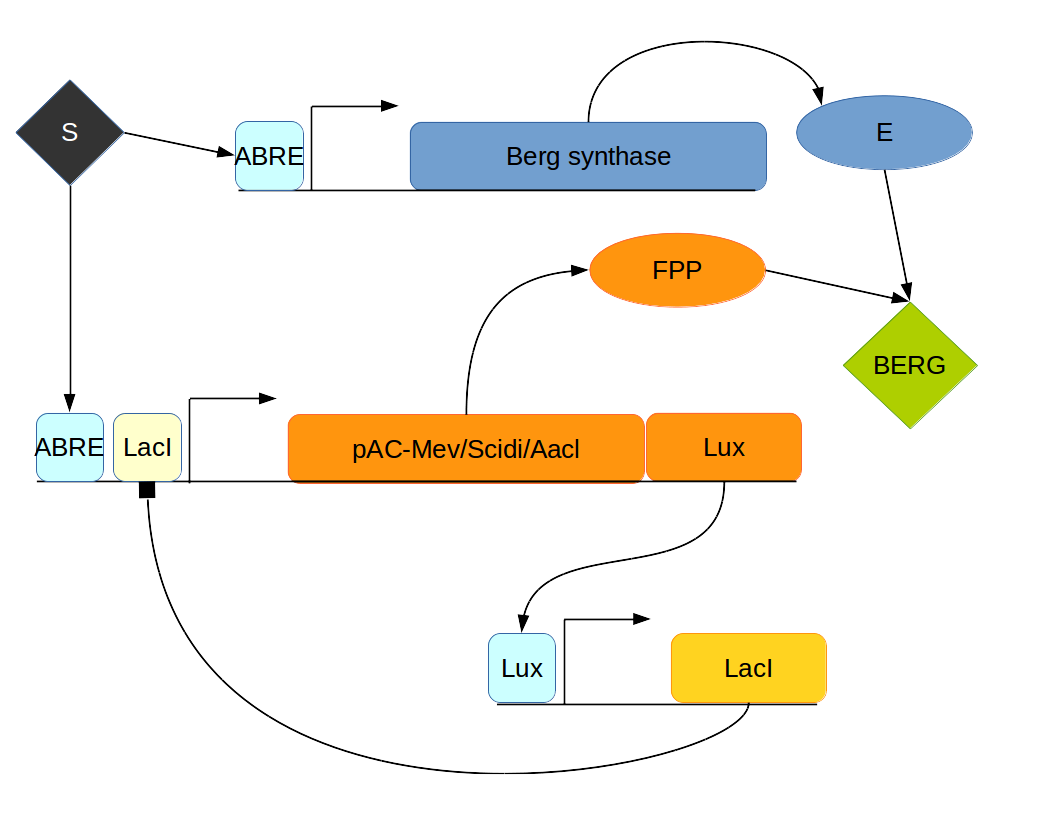
\includegraphics[width=0.5\textwidth]{circuit.png}
\caption{\label{fig:Circuit}This is a figure caption.}
\end{figure}

\subsection{Ecuaciones de Hill}

Para la parte de ... consideramos que el ADN total $\text{D}_{\text{T}}$ es constante, es decir

\begin{align}
\ce{[Z] + [A] <=>[\ce{\hat{k}_+}][\ce{\hat{k}_-}] [ZA] ->[\ce{\hat{k}_{cat}}] [Z]+[F]}\\
\ce{[E] + [F] <=>[\ce{k_+}][\ce{k_-}] [ZA] ->[\ce{k_{cat}}] [Z]+[F]}
\end{align}

Seg\'un las ecuaciones qu\'imicas, las ecuaciones diferenciales para [B], [F], [ZA] y [EF] so

\begin{align}
  \dot{[B]} &= k_{\text{cat}}[E][F]-\gamma_BB \label{eq:Bdot}\\
  \dot{[ZA]} &= \hat{k}_+[Z][A] - \hat{k}_-[ZA]-\hat{k}_{\text{cat}}[ZA] \label{eq:ZAdot}\\
  \dot{[EF]} &= k_+[E][F]-k_-[EF]-k_{\text{cat}}[EF] \label{eq:EFdot}\\
  \dot{[F]} &= -k_+[E][F]+k_-[EF]+\hat{k}_{\text{cat}}[ZA] \label{eq:Fdot}
\end{align}

Asumiendo que los complejos enzima-sustrato est\'an en equilibrio, es decir, $\dot{[ZA]} = 0$ y $\dot{[EF]} = 0$ obtenemos de las ecuaciones \cite{eq:ZAdot} y \cite{eq:EFdot}



Donde a la ecuaci\'on para B se le puso un t\'ermino de degradamiento, pues en las dem\'as como las tasas de reacciones enzim\'aticas son mucho mayores a las de degradamiento blabla

$$[\text{D}_{\text{T}}]=[\text{D}]+[\text{DS}]+[\text{DI}]+[\text{DIS}]$$,

donde $[\text{D}]$ representa el ADN libre, $[\text{DIS}]$ el ADN unido al represor I y al activador S, $[\text{DS}]$ el unido al activador y $[\text{DI}]$ el unido al represor.

En equilibrio y utilizando balance detallado obtenemos las siguientes ecuaciones diferenciales para la concentraci\'on de la enzima $Z$ y su ARN $r_Z$, y de igual manera para la enzima $E$ :

\begin{multline}
\dot{r_Z}(t) = 
\alpha_{IS}
+ \frac{\beta_{IS_I}}{\left( \frac{K_I}{I} \right)^{n_I} + 1 + \left( \frac{S}{K_S} \right)^{n_S} \left( \frac{K_I}{I} \right)^{n_I} + \left( \frac{S}{K_S} \right)^{n_S}}
+ \frac{\beta_{IS_S}}{\left( \frac{K_S}{S} \right)^{n_S} + \left( \frac{I}{K_I} \right)^{n_I} \left( \frac{K_S}{S} \right)^{n_S} + 1 + \left( \frac{I}{K_I} \right)^{n_I}}\\
+ \frac{\beta_{IS_{IS}}}{\left( \frac{K_I}{I} \right)^{n_I} \left( \frac{K_S}{S} \right)^{n_S} + \left( \frac{K_S}{S} \right)^{n_S} + \left( \frac{K_I}{I} \right)^{n_I} + 1}
- \gamma_{r_Z} r_Z
\end{multline}

\begin{align}
\dot{Z}(t) &= k_Z r_Z - \gamma_Z Z\\
\dot{r_E}(t) &= \alpha_S + \frac{\beta_S}{1+ \left( \frac{K_S}{S}\right)^{n_S}} - \gamma_{r_E} r_E\\
\dot{E}(t) &= k_E r_E - \gamma_EE
\end{align}

\subsection{Comments}

Comments can be added to the margins of the document using the \todo{Here's a comment in the margin!} todo command, as shown in the example on the right. You can also add inline comments too:

\todo[inline, color=green!40]{This is an inline comment.}

\subsection{Tables and Figures}

Use the table and tabular commands for basic tables --- see Table~\ref{tab:widgets}, for example. You can upload a figure (JPEG, PNG or PDF) using the files menu. To include it in your document, use the includegraphics command as in the code for Figure~\ref{fig:Circuit} below.

% Commands to include a figure:

\begin{table}
\centering
\begin{tabular}{l|r}
Item & Quantity \\\hline
Widgets & 42 \\
Gadgets & 13
\end{tabular}
\caption{\label{tab:widgets}An example table.}
\end{table}

\subsection{Mathematics}

\LaTeX{} is great at typesetting mathematics. Let $X_1, X_2, \ldots, X_n$ be a sequence of independent and identically distributed random variables with $\text{E}[X_i] = \mu$ and $\text{Var}[X_i] = \sigma^2 < \infty$, and let
$$S_n = \frac{X_1 + X_2 + \cdots + X_n}{n}
      = \frac{1}{n}\sum_{i}^{n} X_i$$
denote their mean. Then as $n$ approaches infinity, the random variables $\sqrt{n}(S_n - \mu)$ converge in distribution to a normal $\mathcal{N}(0, \sigma^2)$.

\subsection{Lists}

You can make lists with automatic numbering \dots

\begin{enumerate}
\item Like this,
\item and like this.
\end{enumerate}
\dots or bullet points \dots
\begin{itemize}
\item Like this,
\item and like this.
\end{itemize}

We hope you find write\LaTeX\ useful, and please let us know if you have any feedback using the help menu above.

\bibliographystyle{plain}
\bibliography{written.bib}

\end{document}
